\subsubsection{Users}

\begin{center}
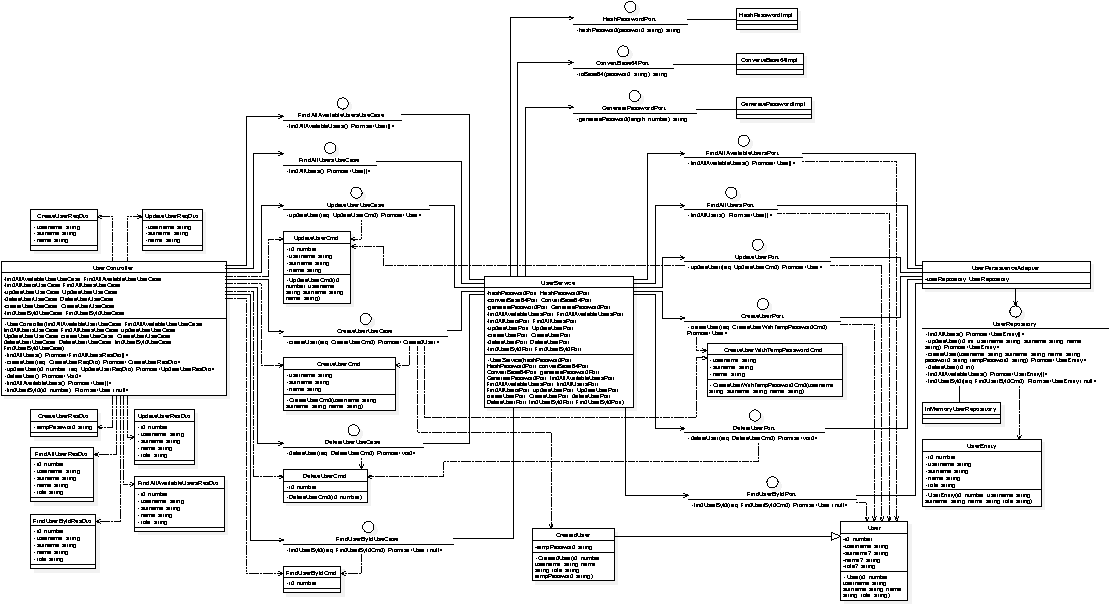
\includegraphics[width=\textwidth]{./backend/users/users.pdf}
\captionof{figure}{\href{https://snakebyteteam.github.io/3-PB/Documenti_esterni/Specifica_tecnica/backend/users/users.pdf}{Diagramma delle classi del modulo Users}}
\end{center}

\addAtr{+}{username: string}{Username dell'utente}
\addAtr{+}{surname: string}{Cognome dell'utente}
\addAtr{+}{name: string}{Nome dell'utente}
\addAtr{+}{tempPassword: string}{Password temporanea generata da assegnare all'utente}
\makeCl{CreateUserWithTempPasswordCmd}{Comando applicativo per la creazione di un utente con password temporanea già generata.}

\addAtr{}{username: string}{Username da assegnare al nuovo utente}
\addAtr{}{surname: string}{Cognome del nuovo utente}
\addAtr{}{name: string}{Nome del nuovo utente}
\makeCl{CreateUserReqDto}{DTO di richiesta per la creazione di un nuovo utente}

\addAtr{}{username: string}{Nuovo username da assegnare all'utente}
\addAtr{}{surname: string}{Nuovo cognome dell'utente}
\addAtr{}{name: string}{Nuovo nome dell'utente}
\makeCl{UpdateUserReqDto}{DTO di richiesta per l'aggiornamento dei dati di un utente esistente}

\addAtr{+}{id: number}{Identificativo dell'utente da aggiornare}
\addAtr{+}{username: string}{Nuovo username dell'utente}
\addAtr{+}{surname: string}{Nuovo cognome dell'utente}
\addAtr{+}{name: string}{Nuovo nome dell'utente}
\makeCl{UpdateUserCmd}{Comando applicativo per l'aggiornamento dei dati di un utente.}

\addAtr{}{id: number}{Identificativo univoco dell'utente}
\addAtr{}{username: string}{Username dell'utente}
\addAtr{}{surname: string}{Cognome dell'utente}
\addAtr{}{name: string}{Nome dell'utente}
\addAtr{}{role: string}{Ruolo dell'utente nel sistema}
\makeCl{FindAllAvailableUsersResDto}{DTO di risposta per un elemento della lista degli utenti disponibili per l'assegnazione}

\addAtr{}{id: number}{Identificativo univoco dell'utente}
\addAtr{}{username: string}{Username dell'utente}
\addAtr{}{surname: string}{Cognome dell'utente}
\addAtr{}{name: string}{Nome dell'utente}
\addAtr{}{role: string}{Ruolo dell'utente nel sistema}
\makeCl{FindAllUserResDto}{DTO di risposta per un elemento della lista di tutti gli utenti del sistema}

\addAtr{}{id: number}{Identificativo univoco dell'utente}
\addAtr{}{username: string}{Username dell'utente}
\addAtr{}{surname: string}{Cognome dell'utente}
\addAtr{}{name: string}{Nome dell'utente}
\addAtr{}{role: string}{Ruolo dell'utente nel sistema}
\makeCl{FindUserByIdResDto}{DTO di risposta contenente i dettagli di un singolo utente}

\addAtr{}{id: number}{Identificativo univoco dell'utente aggiornato}
\addAtr{}{username: string}{Username aggiornato}
\addAtr{}{surname: string}{Cognome aggiornato}
\addAtr{}{name: string}{Nome aggiornato}
\addAtr{}{role: string}{Ruolo dell'utente nel sistema}
\makeCl{UpdateUserResDto}{DTO di risposta restituito dopo l'aggiornamento di un utente}

\addAtr{}{username: number}{Username assegnato al nuovo utente}
\addAtr{}{surname: string}{Cognome del nuovo utente}
\addAtr{}{role: string}{Ruolo assegnato al nuovo utente}
\addAtr{}{name: string}{Nome del nuovo utente}
\addAtr{}{tempPassword: string}{Password temporanea generata per il primo accesso}
\makeCl{CreateUserResDto}{DTO di risposta restituito dopo la creazione di un nuovo utente, include la password temporanea}

% model

\addAtr{+}{id: number}{Identificativo univoco dell'utente appena creato}
\addAtr{+}{username: string}{Username dell'utente appena creato}
\addMet{+}{getTempPassword(): string $|$ undefined}{Restituisce la password temporanea generata, undefined se non disponibile}
\makeCl{CreatedUser}{Modello di dominio che rappresenta un utente appena creato, con la relativa password temporanea}

\addAtr{-}{id: number}{Identificativo univoco dell'utente}
\addAtr{-}{username: string}{Username dell'utente}
\addMet{+}{getId(): number}{Restituisce l'identificativo univoco dell'utente}
\addMet{+}{getUsername(): string}{Restituisce lo username dell'utente}
\addMet{+}{getSurname(): string $|$ undefined}{Restituisce il cognome dell'utente, undefined se non impostato}
\addMet{+}{getName(): string $|$ undefined}{Restituisce il nome dell'utente, undefined se non impostato}
\addMet{+}{getRole(): string $|$ undefined}{Restituisce il ruolo dell'utente, undefined se non impostato}
\makeCl{User}{Modello di dominio che rappresenta un utente del sistema}

% controller

\addAtr{-}{findAllUsersUseCase: FindAllUsersUseCase}{Use case per il recupero di tutti gli utenti}
\addAtr{-}{findUserByIdUseCase: FindUserByIdUseCase}{Use case per il recupero di un utente tramite identificativo}
\addAtr{-}{findAllAvailableUsersUseCase: FindAllAvailableUsersUseCase}{Use case per il recupero degli utenti disponibili per l'assegnazione}
\addAtr{-}{updateUserUseCase: UpdateUserUseCase}{Use case per l'aggiornamento dei dati di un utente}
\addAtr{-}{createUserUseCase: CreateUserUseCase}{Use case per la creazione di un nuovo utente}
\addAtr{-}{deleteUserUseCase: DeleteUserUseCase}{Use case per l'eliminazione di un utente}
\addMet{+}{findAllUsers(): Promise$<$FindAllUserResDto[]$>$}{Espone l'endpoint per il recupero di tutti gli utenti del sistema}
\addMet{+}{findAllAvailableUsers(): Promise$<$FindAllAvailableUsersResDto[]$>$}{Espone l'endpoint per il recupero degli utenti disponibili per l'assegnazione}
\makeCl{UsersController}{Controller REST che gestisce le richieste HTTP relative agli utenti}

% command

\addAtr{+}{username: string}{Username da assegnare al nuovo utente}
\addAtr{+}{surname: string}{Cognome del nuovo utente}
\addAtr{+}{name: string}{Nome del nuovo utente}
\makeCl{CreateUserCmd}{Comando per la creazione di un nuovo utente}

\addAtr{+}{username: string}{Username da assegnare al nuovo utente}
\addAtr{+}{surname: string}{Cognome del nuovo utente}
\addAtr{+}{name: string}{Nome del nuovo utente}
\addAtr{+}{tempPassword: string}{Password temporanea generata per il primo accesso}
\makeCl{CreateUserWithTempPasswordCmd}{Comando per la creazione di un utente comprensivo di password temporanea già generata}

\addAtr{+}{id: number}{Identificativo dell'utente da eliminare}
\makeCl{DeleteUserCmd}{Comando per l'eliminazione di un utente}

\addAtr{+}{id: number}{Identificativo dell'utente da recuperare}
\makeCl{FindUserByIdCmd}{Comando per il recupero di un utente tramite identificativo}

\addAtr{+}{id: number}{Identificativo dell'utente da aggiornare}
\addAtr{+}{username: string}{Nuovo username da assegnare}
\addAtr{+}{surname: string}{Nuovo cognome da assegnare}
\addAtr{+}{name: string}{Nuovo nome da assegnare}
\makeCl{UpdateUserCmd}{Comando per l'aggiornamento dei dati anagrafici di un utente}

% use case

\addMet{+}{createUser(req: CreateUserCmd): Promise$<$CreatedUser$>$}{Crea un nuovo utente generando una password temporanea e restituisce il modello dell'utente creato}
\makeItf{CreateUserUseCase}{Interfaccia del use case per la creazione di un nuovo utente}

\addMet{+}{deleteUser(req: DeleteUserCmd): Promise$<$void$>$}{Elimina l'utente identificato dal comando}
\makeItf{DeleteUserUseCase}{Interfaccia del use case per l'eliminazione di un utente}

\addMet{+}{findAllAvailableUsers(): Promise$<$User[]$>$}{Recupera tutti gli utenti disponibili per l'assegnazione a un ward}
\makeItf{FindAllAvailableUsersUseCase}{Interfaccia del use case per il recupero degli utenti disponibili}

\addMet{+}{findAllUsers(): Promise$<$User[]$>$}{Recupera tutti gli utenti registrati nel sistema}
\makeItf{FindAllUsersUseCase}{Interfaccia del use case per il recupero di tutti gli utenti}

\addMet{+}{findUserById(req: FindUserByIdCmd): Promise$<$User $|$ null$>$}{Recupera un utente tramite identificativo, restituisce null se non trovato}
\makeItf{FindUserByIdUseCase}{Interfaccia del use case per il recupero di un singolo utente}

\addMet{+}{updateUser(req: UpdateUserCmd): Promise$<$User$>$}{Aggiorna i dati anagrafici dell'utente e restituisce il modello aggiornato}
\makeItf{UpdateUserUseCase}{Interfaccia del use case per l'aggiornamento dei dati di un utente}

% service

\addAtr{-}{findAllUsersPort: FindAllUsersPort}{Porta per il recupero di tutti gli utenti}
\addAtr{-}{findUserByIdPort: FindUserByIdPort}{Porta per il recupero di un utente tramite identificativo}
\addAtr{-}{findAllAvailableUsersPort: FindAllAvailableUsersPort}{Porta per il recupero degli utenti disponibili}
\addAtr{-}{generatePasswordPort: GeneratePasswordPort}{Porta per la generazione di password temporanee}
\addAtr{-}{hashPasswordPort: HashPasswordPort}{Porta per l'hashing delle password}
\addAtr{-}{convertBase64Port: ConvertBase64Port}{Porta per la conversione delle password in formato Base64}
\addMet{+}{findAllUsers(): Promise$<$User[]$>$}{Recupera tutti gli utenti delegando alla porta di persistenza}
\addMet{+}{findUserById(req: FindUserByIdCmd): Promise$<$User $|$ null$>$}{Recupera un utente per identificativo delegando alla porta di persistenza}
\addMet{+}{findAllAvailableUsers(): Promise$<$User[]$>$}{Recupera gli utenti disponibili delegando alla porta di persistenza}
\addMet{+}{updateUser(req: UpdateUserCmd): Promise$<$User$>$}{Aggiorna i dati di un utente delegando alla porta di persistenza}
\addMet{+}{createUser(req: CreateUserCmd): Promise$<$CreatedUser$>$}{Genera una password temporanea, la codifica e crea il nuovo utente tramite le porte di persistenza}
\addMet{+}{deleteUser(req: DeleteUserCmd): Promise$<$void$>$}{Elimina un utente delegando alla porta di persistenza}
\makeCl{UsersService}{Servizio applicativo che implementa i use case relativi alla gestione degli utenti}

% port

\addMet{+}{toBase64(password: string): string}{Codifica la password fornita in formato Base64}
\addMet{+}{toPlain(password: string): string}{Decodifica una password da formato Base64 al testo in chiaro}
\makeItf{ConvertBase64Port}{Porta di uscita per la conversione delle password da e verso il formato Base64}

\addMet{+}{createUser(req: CreateUserWithTempPasswordCmd): Promise$<$User$>$}{Persiste il nuovo utente con la password temporanea e restituisce il modello creato}
\makeItf{CreateUserPort}{Porta di uscita per la creazione e persistenza di un nuovo utente}

\addMet{+}{deleteUser(req: DeleteUserCmd): Promise$<$void$>$}{Elimina l'utente specificato dal livello di persistenza}
\makeItf{DeleteUserPort}{Porta di uscita per l'eliminazione di un utente}

\addMet{+}{findAllAvailableUsers(): Promise$<$User[]$>$}{Recupera dal livello di persistenza gli utenti non ancora assegnati a un ward}
\makeItf{FindAllAvailableUsersPort}{Porta di uscita per il recupero degli utenti disponibili per l'assegnazione}

\addMet{+}{findAllUsers(): Promise$<$User[]$>$}{Recupera dal livello di persistenza tutti gli utenti del sistema}
\makeItf{FindAllUsersPort}{Porta di uscita per il recupero di tutti gli utenti}

\addMet{+}{findUserById(req: FindUserByIdCmd): Promise$<$User $|$ null$>$}{Recupera dal livello di persistenza un utente per identificativo, restituisce null se non trovato}
\makeItf{FindUserByIdPort}{Porta di uscita per il recupero di un singolo utente tramite identificativo}

\addMet{+}{hashPassword(password: string): string}{Applica una funzione di hashing alla password e restituisce il digest risultante}
\makeItf{HashPasswordPort}{Porta di uscita per l'hashing sicuro delle password}

\addMet{+}{generatePassword(length: number): string}{Genera una password casuale della lunghezza specificata}
\makeItf{GeneratePasswordPort}{Porta di uscita per la generazione di password temporanee casuali}

\addMet{+}{updateUser(req: UpdateUserCmd): Promise$<$User$>$}{Aggiorna i dati dell'utente nel livello di persistenza e restituisce il modello aggiornato}
\makeItf{UpdateUserPort}{Porta di uscita per l'aggiornamento dei dati di un utente}

% entity

\addAtr{+}{id: number}{Identificativo univoco dell'utente nel database}
\addAtr{+}{username: string}{Username dell'utente}
\addAtr{+}{surname: string}{Cognome dell'utente}
\addAtr{+}{name: string}{Nome dell'utente}
\addAtr{+}{role: string}{Ruolo dell'utente nel sistema}
\makeCl{UserEntity}{Entità di persistenza che rappresenta un utente nel database}

% adapter

\addAtr{-}{userRepository: UserRepository}{Repository per l'accesso ai dati degli utenti nel database}
\addMet{+}{createUser(req: CreateUserWithTempPasswordCmd): Promise$<$User$>$}{Delega al repository la creazione dell'utente e mappa il risultato nel modello di dominio}
\addMet{+}{updateUser(req: UpdateUserCmd): Promise$<$User$>$}{Delega al repository l'aggiornamento dell'utente e mappa il risultato nel modello di dominio}
\addMet{+}{findUserById(req: FindUserByIdCmd): Promise$<$User $|$ null$>$}{Recupera e mappa un utente per identificativo dal repository}
\addMet{+}{findAllUsers(): Promise$<$User[]$>$}{Recupera e mappa tutti gli utenti dal repository}
\addMet{+}{findAllAvailableUsers(): Promise$<$User[]$>$}{Recupera e mappa gli utenti disponibili dal repository}
\addMet{+}{deleteUser(req: DeleteUserCmd): Promise$<$void$>$}{Delega al repository l'eliminazione dell'utente specificato}
\makeCl{UserPersistenceAdapter}{Adattatore di persistenza che implementa le porte relative agli utenti}

% repository

\addMet{+}{createUser(username: string, surname: string, name: string, tempPassword: string): Promise$<$UserEntity$>$}{Inserisce un nuovo utente nel database con i dati e la password temporanea forniti}
\addMet{+}{deleteUser(id: number): Promise$<$void$>$}{Elimina dal database l'utente con l'identificativo specificato}
\addMet{+}{findAllAvailableUsers(): Promise$<$UserEntity[]$>$}{Recupera dal database gli utenti non ancora assegnati a un ward}
\addMet{+}{findAllUsers(): Promise$<$UserEntity[]$>$}{Recupera dal database tutti gli utenti del sistema}
\addMet{+}{updateUser(id: number, username: string, surname: string, \\ name: string): Promise$<$UserEntity$>$}{Aggiorna nel database i dati anagrafici dell'utente specificato}
\addMet{+}{findUserById(id: number): Promise$<$UserEntity $|$ null$>$}{Recupera dal database un utente per identificativo, restituisce null se non trovato}
\makeItf{UserRepository}{Interfaccia del repository per le operazioni di persistenza relative agli utenti}

% repository impl

\addMet{+}{findAllUsers(): Promise$<$UserEntity[]$>$}{Implementa il recupero di tutti gli utenti tramite query al database}
\addMet{+}{findUserById(id: number): Promise$<$UserEntity $|$ null$>$}{Implementa il recupero di un utente per identificativo tramite query al database}
\addMet{+}{findAllAvailableUsers(): Promise$<$UserEntity[]$>$}{Implementa il recupero degli utenti disponibili tramite query al database}
\addMet{+}{updateUser(id: number, username: string, \\ surname: string, name: string): Promise$<$UserEntity$>$}{Implementa l'aggiornamento dei dati anagrafici di un utente tramite query al database}
\addMet{+}{createUser(username: string, surname: string, name: string, tempPassword: string): Promise$<$UserEntity$>$}{Implementa l'inserimento di un nuovo utente nel database}
\addMet{+}{deleteUser(id: number): Promise$<$void$>$}{Implementa l'eliminazione di un utente tramite query al database}
\makeCl{UsersRepositoryImpl}{Implementazione concreta del repository per gli utenti}
